\chapter{A APROXIMAÇÃO DE TEMPO DE TRÂNSITO ERC}
\label{ap:tempo_cre}

\begin{figure}[H]
\caption{Geometria do arranjo ERC.}
\begin{center}
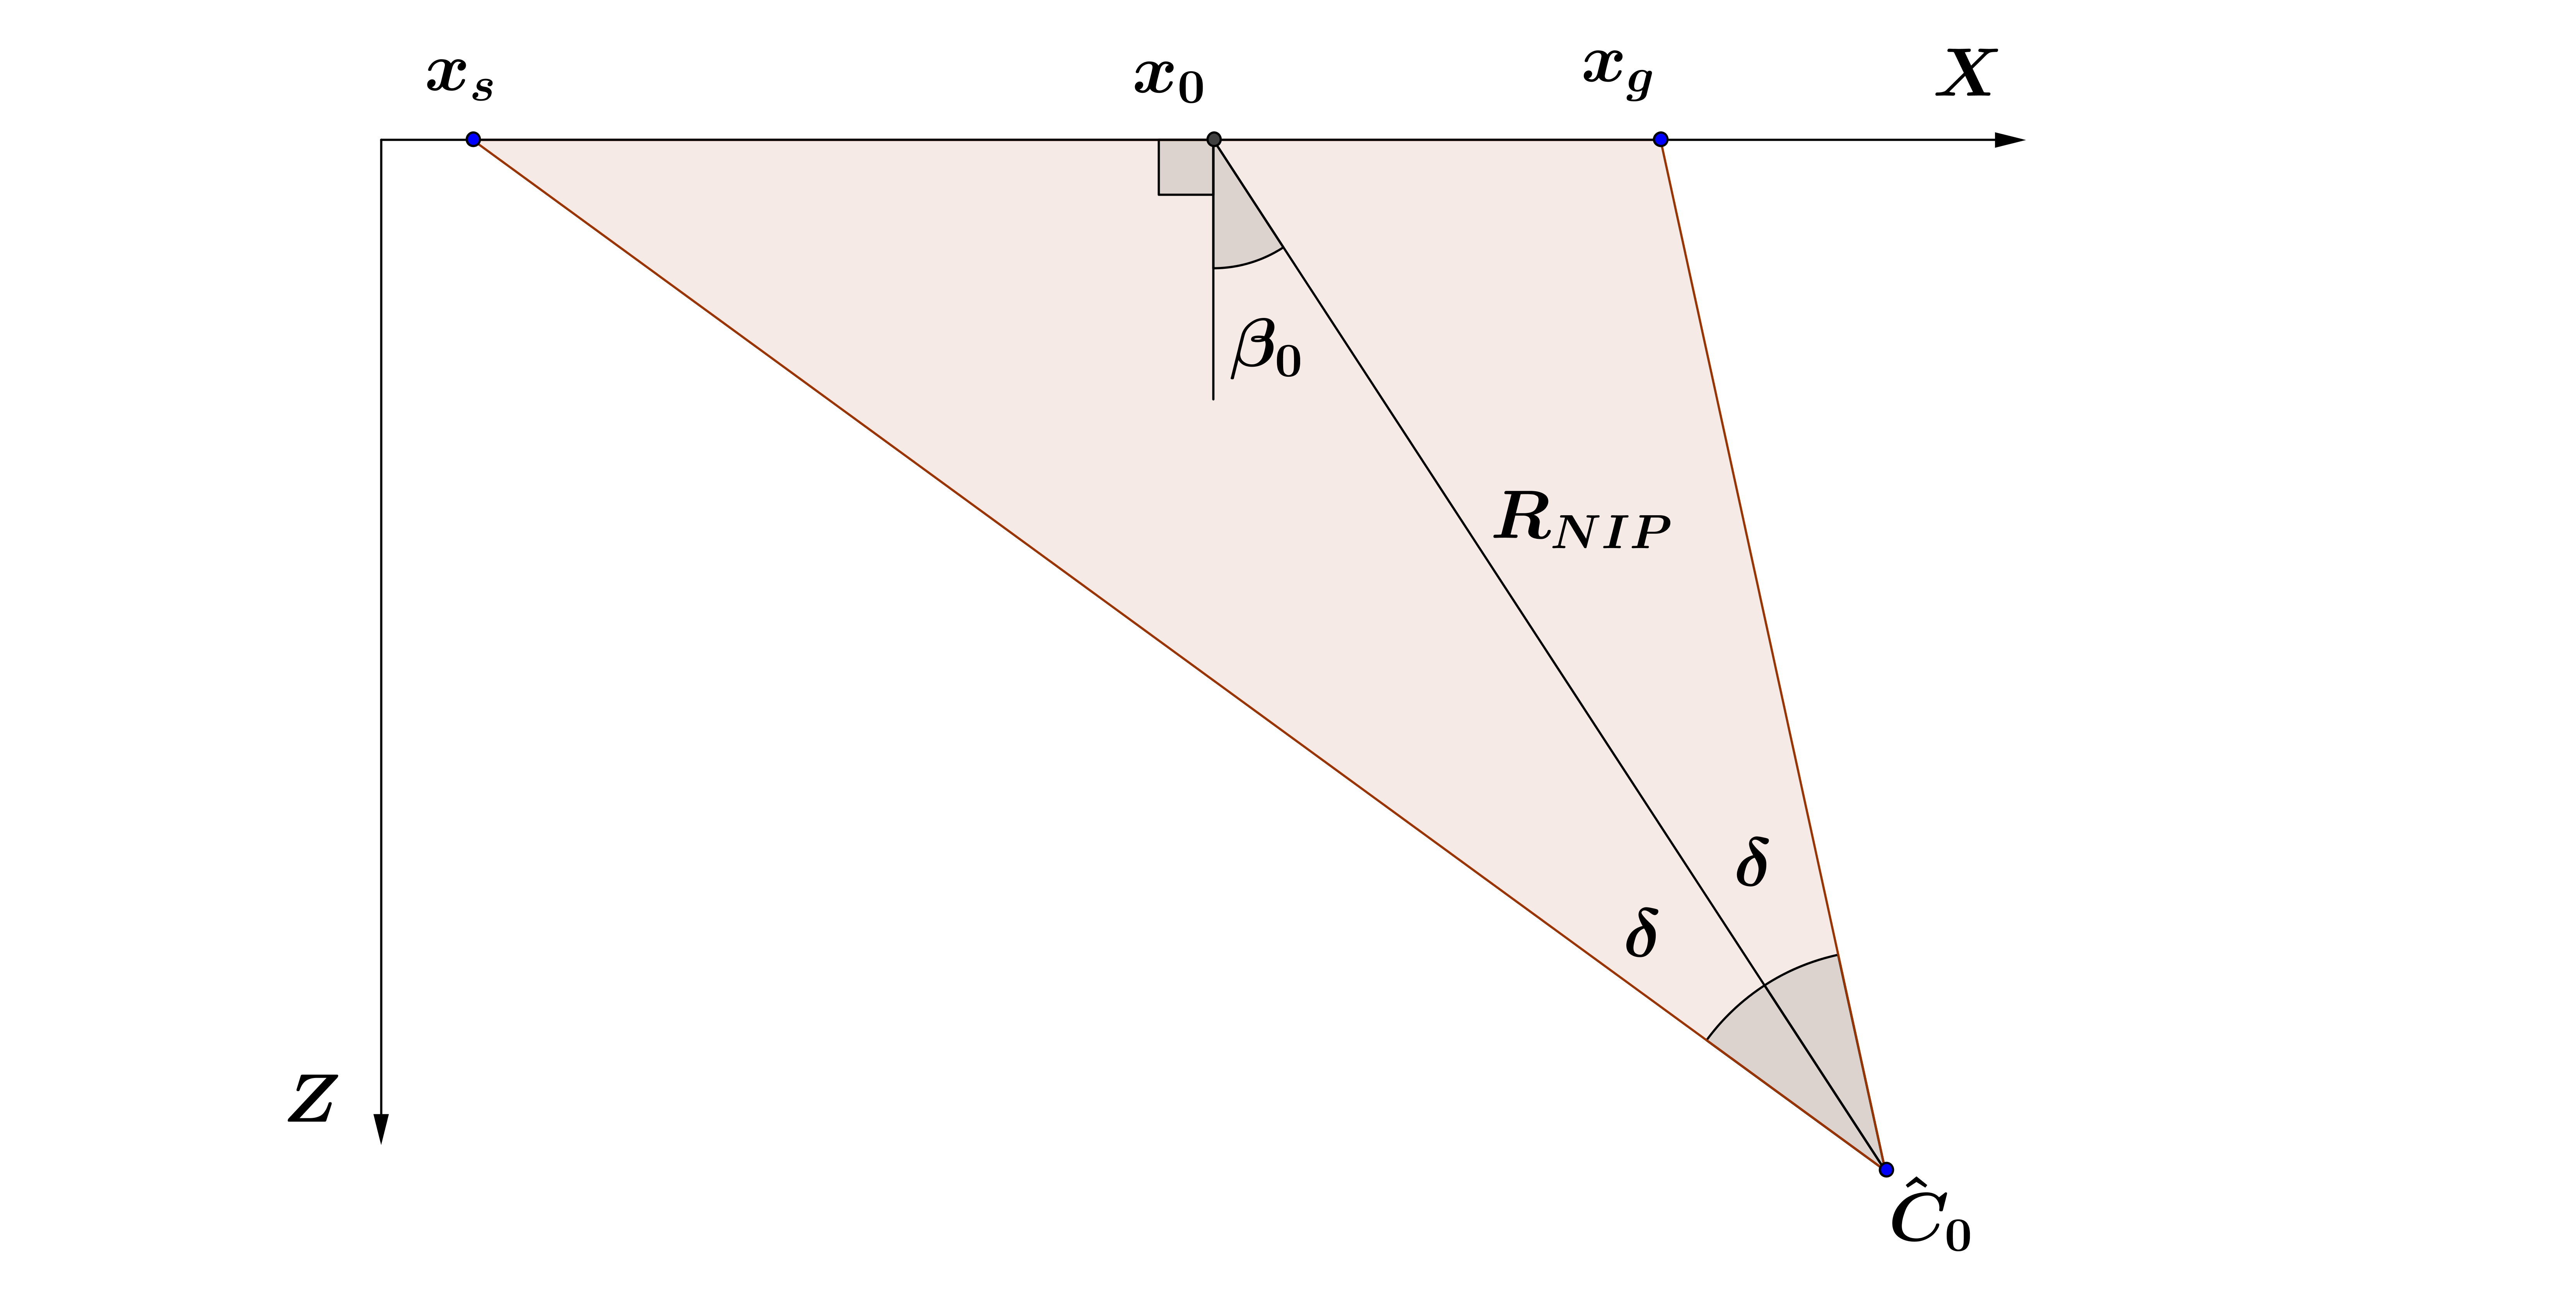
\includegraphics[scale=0.5]{images/creGeom.png}
\vspace{-0.3cm}
\end{center}
\begin{center}
 Fonte: Do Autor.
\end{center}
\label{fig:ap:1.1}
\end{figure}

A expressão genérica do sobretempo normal do ERC:

\begin{equation}
\label{eq:ap:1.1}
\tau = \tau_0 + \Delta \tau_{ERC}
\end{equation}

Onde:

\begin{equation}
\label{eq:ap:1.2}
\Delta \tau_{ERC} = \Delta \tau_s + \Delta \tau_g
\end{equation}

Definindo:

\begin{equation}
\label{eq:ap:1.3}
\Delta x_s = x_s - x_0
\end{equation}

\begin{equation}
\label{eq:ap:1.4}
\Delta x_g = x_g - x_0
\end{equation}

Definindo os tempos $\Delta \tau_s$ e $\Delta \tau_g$ a partir da geometria na Figura \ref{fig:ap:1.1}:

\begin{equation}
\label{eq:ap:1.5}
\Delta \tau_s = \left( \frac{\overline{\hat{C_0}S}}{v_0} - \frac{\overline{\hat{C_0}x_0}}{v_0} \right)
\end{equation}

\begin{equation}
\label{eq:ap:1.6}
\Delta \tau_g = \left( \frac{\overline{\hat{C_0}G}}{v_0} - \frac{\overline{\hat{C_0}x_0}}{v_0} \right)
\end{equation}

\begin{figure}[H]
\caption{Triângulo genérico para aplicação da lei dos cossenos.}
\begin{center}
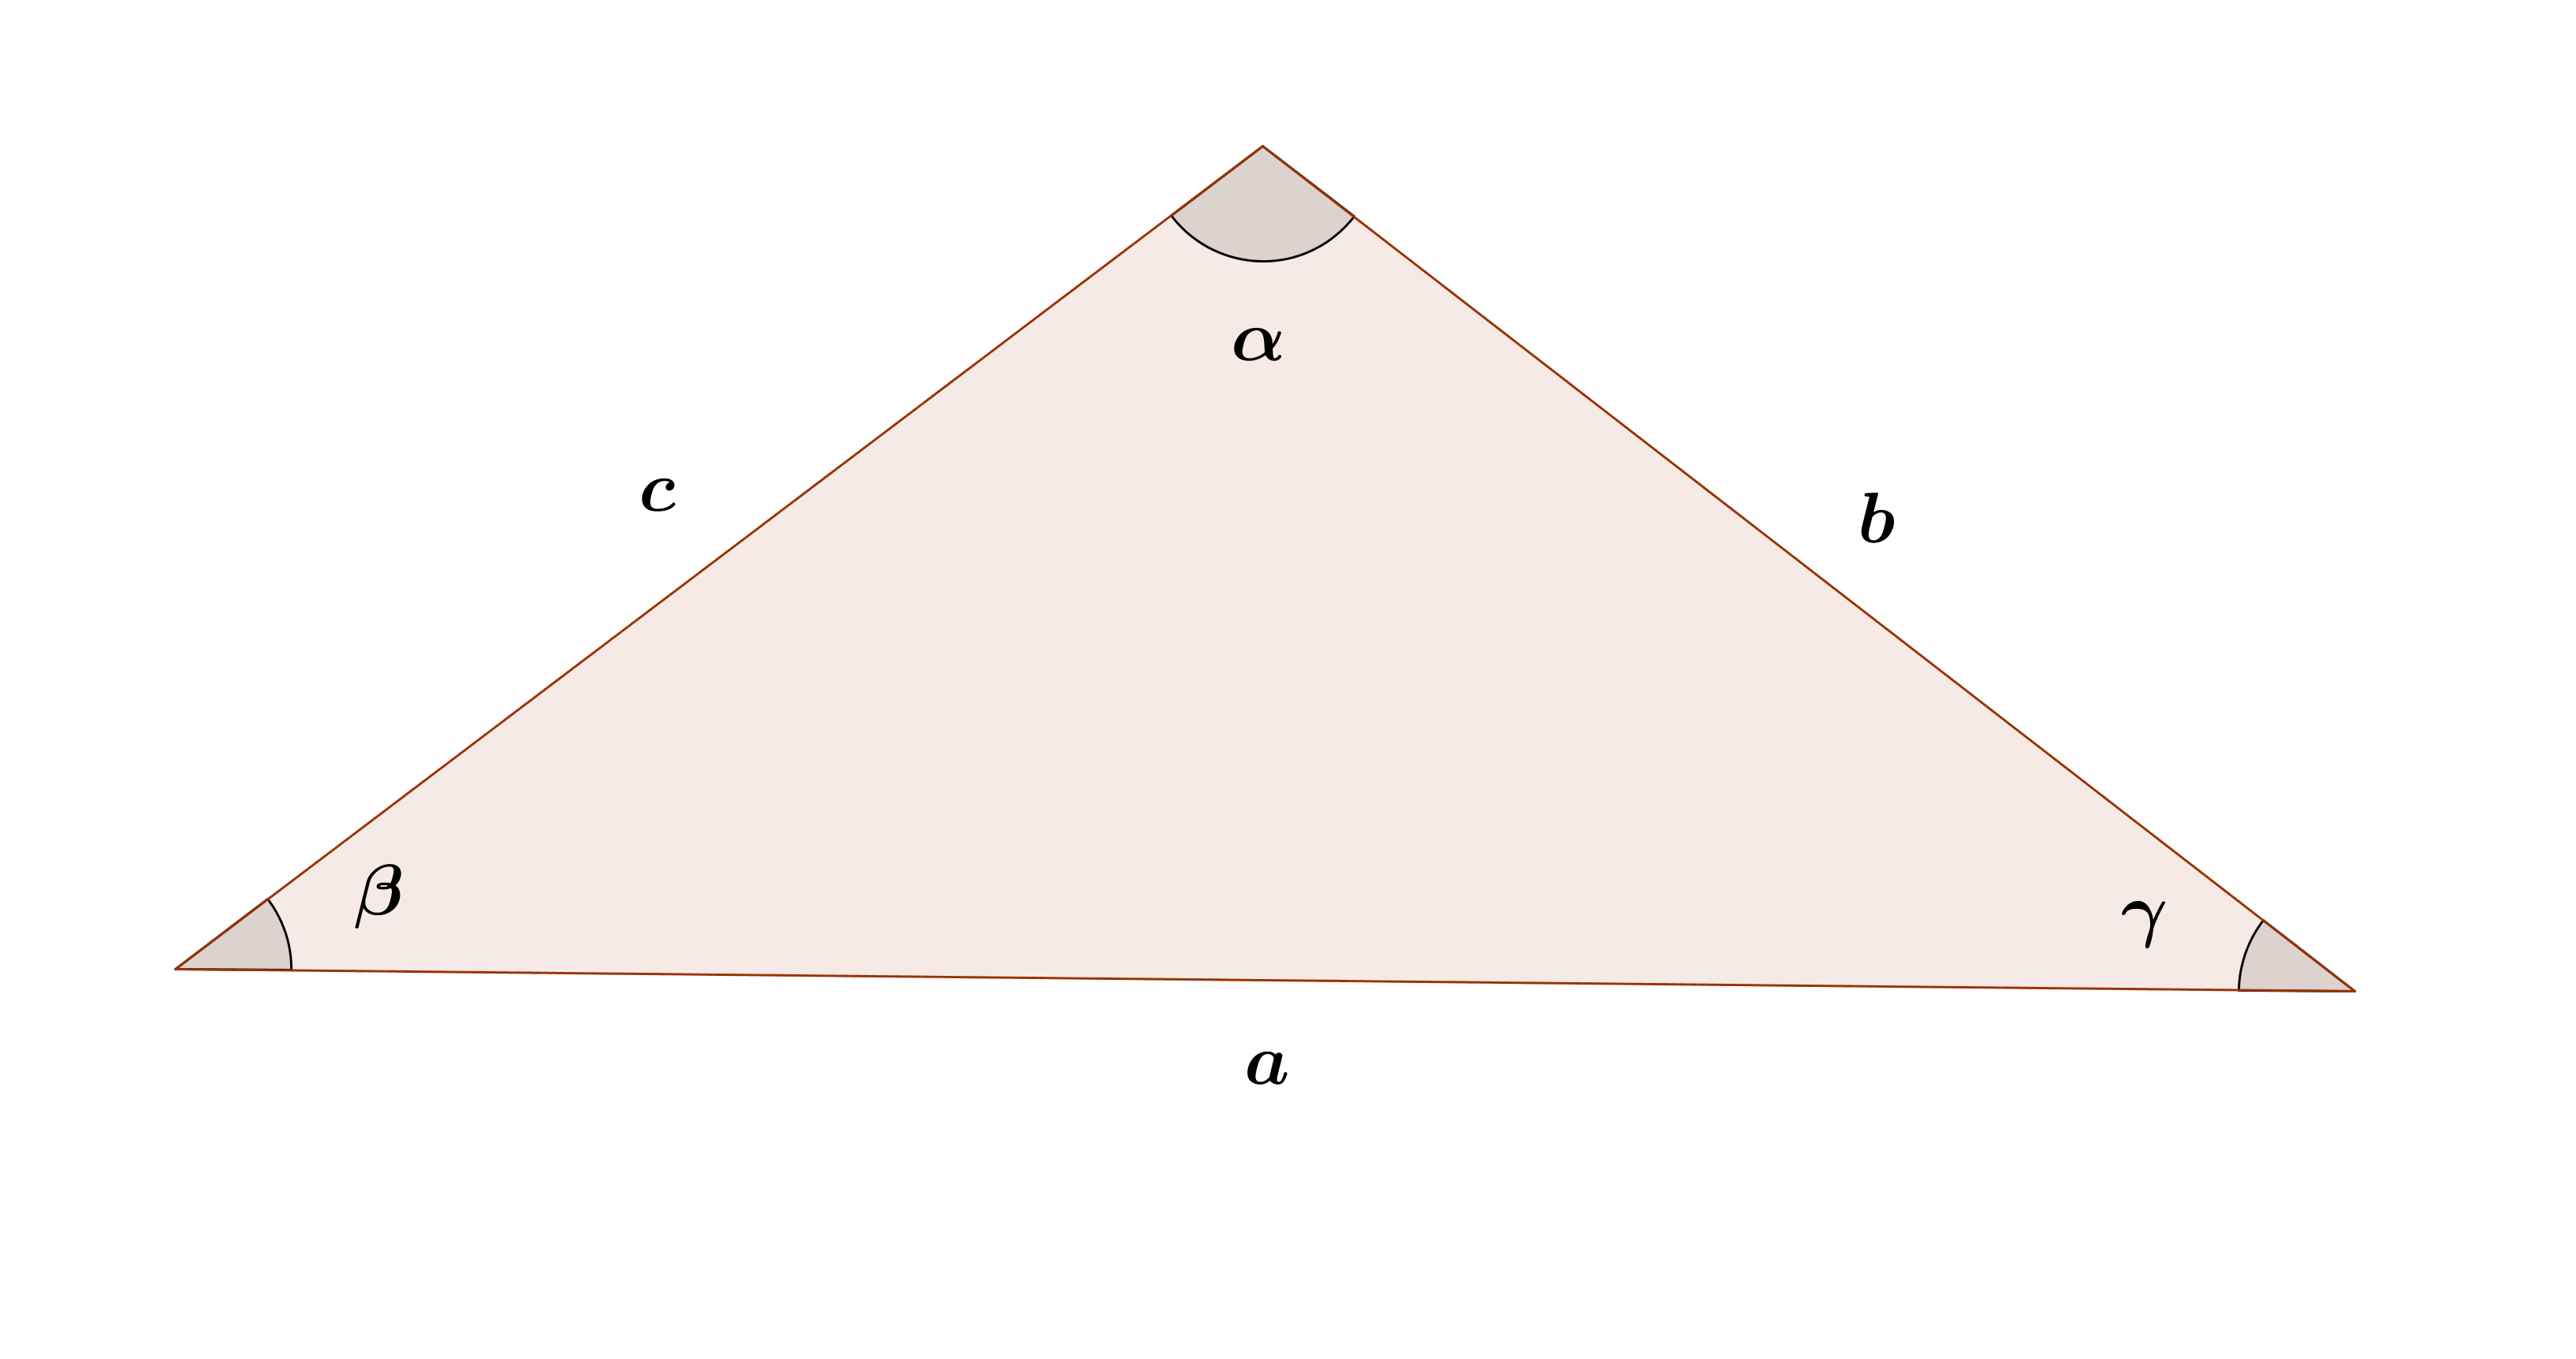
\includegraphics[scale=0.8]{images/leiCossenos.png}
\vspace{-0.3cm}
\end{center}
\begin{center}
 Fonte: Do Autor.
\end{center}
\label{fig:ap:1.2}
\end{figure}

Relembrando a lei dos cossenos a partir da Figura \ref{fig:ap:1.2}:

\begin{equation}
 \label{eq:ap:1.7}
 a^2 = b^2 + c^2 - 2 b c \cos{\alpha}
\end{equation}

\begin{equation}
 \label{eq:ap:1.8}
 b^2 = a^2 + c^2 - 2 a c \cos{\beta}
\end{equation}

\begin{equation}
 \label{eq:ap:1.9}
 c^2 = a^2 + b^2 - 2 a b \cos{\gamma}
\end{equation}

Com auxílio da lei dos cossenos podemos definir os comprimentos:

\begin{equation}
 \label{eq:ap:1.10}
 \overline{\hat{C_0}S}^2 = \Delta x_{s}^2 + R_{NIP}^2 - 2 \Delta x_s R_{NIP} \cos{\beta_0 + \frac{\pi}{2}}
\end{equation}

\begin{equation}
 \label{eq:ap:1.11}
 \cos{\left( \beta_0 + \frac{\pi}{2} \right)} 
 = \cos{\beta_0} \cos{\frac{\pi}{2}} - \sin{\beta_0} \sin{\frac{\pi}{2}}
\end{equation}

Como o $\cos{\frac{\pi}{2}}=0$ e $\sin{\frac{\pi}{2}}=1$:

\begin{equation}
 \label{eq:ap:1.12}
 \overline{\hat{C_0}S}^2 = \Delta x_{s}^2 + R_{NIP}^2 - 2 \Delta x_s R_{NIP} \sin{\beta_0}
\end{equation}

Da mesma forma:

\begin{equation}
 \label{eq:ap:1.13}
 \overline{\hat{C_0}G}^2 = \Delta x_{g}^2 + R_{NIP}^2 - 2 \Delta x_g R_{NIP} \cos{\frac{\pi}{2} - \beta_0}
\end{equation}

\begin{equation}
 \label{eq:ap:1.14}
 \cos{\left( \frac{\pi}{2} - \beta_0 \right)} 
 = \cos{\frac{\pi}{2}} \cos{\beta_0} - \sin{\frac{\pi}{2}} \sin{\beta_0}
\end{equation}

Como o $\cos{\frac{\pi}{2}}=0$ e $\sin{\frac{\pi}{2}}=1$:

\begin{equation}
 \label{eq:ap:1.15}
 \overline{\hat{C_0}G}^2 = \Delta x_{g}^2 + R_{NIP}^2 - 2 \Delta x_g R_{NIP} \sin{\beta_0}
\end{equation}

Então:

\begin{equation}
 \label{eq:ap:1.16}
 \overline{\hat{C_0}S} = \sqrt{ \Delta x_{s}^2 + R_{NIP}^2 - 2 \Delta x_s R_{NIP} \sin{\beta_0} }
\end{equation}

\begin{equation}
 \label{eq:ap:1.17}
 \overline{\hat{C_0}S} = 
 R_{NIP} \sqrt{  1 - 2 \Delta x_s \frac{\sin{\beta_0}}{R_{NIP}} + \frac{\Delta x_{s}^2}{R_{NIP}^2} }
\end{equation}

Da mesma forma:

\begin{equation}
 \label{eq:ap:1.18}
 \overline{\hat{C_0}G} = \sqrt{ \Delta x_{g}^2 + R_{NIP}^2 - 2 \Delta x_g R_{NIP} \sin{\beta_0} }
\end{equation}

\begin{equation}
 \label{eq:ap:1.19}
 \overline{\hat{C_0}G} = 
 R_{NIP} \sqrt{  1 - 2 \Delta x_g \frac{\sin{\beta_0}}{R_{NIP}} + \frac{\Delta x_{g}^2}{R_{NIP}^2} }
\end{equation}

Defindo o comprimento $\overline{\hat{C_0}x_0}$\footnote{O comprimento
$\overline{\hat{C_0}x_0} = R_{NIP}$ não é de nenhuma forma o comprimento do raio normal.}:

\begin{equation}
 \label{eq:ap:1.20}
 \overline{\hat{C_0}x_0} = R_{NIP}
\end{equation}

\begin{equation}
 \label{eq:ap:1.21}
t_0 = \frac{R_{NIP}}{v_0}
\end{equation}

Então, a Equação \ref{eq:ap:1.1} pode ser reescrita como:

\begin{equation}
 \label{eq:ap:1.22}
\tau = \tau_0 + \left( \frac{\overline{\hat{C_0}S}}{v_0} - \frac{\overline{\hat{C_0}x_0}}{v_0} \right)
+ \left( \frac{\overline{\hat{C_0}G}}{v_0} - \frac{\overline{\hat{C_0}x_0}}{v_0} \right)
\end{equation}

\begin{equation}
 \label{eq:ap:1.23}
\tau = \tau_0 + - 2 \frac{\overline{\hat{C_0}x_0}}{v_0} + \frac{\overline{\hat{C_0}S}}{v_0}
+ \frac{\overline{\hat{C_0}G}}{v_0}
\end{equation}

\begin{equation}
 \label{eq:ap:1.24}
\tau = \left( \tau_0 + \frac{2 R_{NIP}}{v_0} \right)
+ \frac{R_{NIP}}{v_0} \left( \sqrt{  1 - 2 \Delta x_s \frac{\sin{\beta_0}}{R_{NIP}} + \frac{\Delta x_{s}^2}{R_{NIP}^2} }
+ \sqrt{  1 - 2 \Delta x_g \frac{\sin{\beta_0}}{R_{NIP}} + \frac{\Delta x_{g}^2}{R_{NIP}^2} } \right)
\end{equation}

Utilizando a definição do meio-afastamento $h$ e do PMC $m$: 

\begin{equation}
 \label{eq:ap:1.25}
 h=(x_g-x_s)/2
\end{equation}

\begin{equation}
 \label{eq:ap:1.26}
 m=(x_g + x_s)/2
\end{equation}

Podemos redefinir $x_g$ e $x_s$ em função de $h$ e $m$:

\begin{equation}
 \label{eq:ap:1.27}
 x_g = 2h + x_s
\end{equation}

\begin{equation}
 \label{eq:ap:1.28}
 x_s = 2m - x_g
\end{equation}

Substituindo a Equação \ref{eq:ap:1.28} em \ref{eq:ap:1.27}:

\begin{equation}
 \label{eq:ap:1.29}
 x_g = 2h + 2m - x_g = m + h
\end{equation}

Substituindo a Equação \ref{eq:ap:1.29} de volta em \ref{eq:ap:1.28}:

\begin{equation}
 \label{eq:ap:1.30}
 x_s = 2m - m -h = m - h
\end{equation}

Retomando as definições de $\Delta x_g$ e de $\Delta x_s$ nas Equações \ref{eq:ap:1.3} e \ref{eq:ap:1.4}
e substituindo os resultados obtidos nas Equações \ref{eq:ap:1.29} e \ref{eq:ap:1.30}:

\begin{equation}
 \label{eq:ap:1.31}
 \Delta x_g = x_g - x_0 = m - x_0 + h
\end{equation}

\begin{equation}
 \label{eq:ap:1.32}
 \Delta x_s = x_s - x_0 = m - x_0 - h
\end{equation}

Se definirmos $x_0$ como um PMC central $m_0$ onde será realizada a aproximação de tempo de trânsito:

\begin{equation}
 \label{eq:ap:1.33}
 \Delta x_g = m - m_0 - h
\end{equation}

\begin{equation}
 \label{eq:ap:1.34}
 \Delta x_s = m - m_0 - h
\end{equation}

Definindo o parâmetro de assimetria $\alpha$ como:

\begin{equation}
 \label{eq:ap:1.35}
 \alpha = \frac{\sin \beta_0}{R_{NIP}}
\end{equation}

Substituindo as definições das Equações \ref{eq:ap:1.33}-\ref{eq:ap:1.35} na
Equação \ref{eq:ap:1.24}, teremos a Equação de tempo de trânsito ERC (Equação \ref{eq:2.3}).